\documentclass[8pt]{article} %{report}
\usepackage{fullpage}
\usepackage{graphicx}
\usepackage{subfigure}
\usepackage{float}
\usepackage[mathletters]{ucs}
\usepackage[utf8x]{inputenc}
\usepackage{multirow}
\usepackage{hyperref}
\usepackage{wrapfig}
\usepackage{tabto}
\usepackage{listings}
\usepackage{color,soul}
\usepackage{subcaption}
\usepackage{amsmath}
\usepackage{mathtools}

\definecolor{dkgreen}{rgb}{0,0.6,0}
\definecolor{gray}{rgb}{0.5,0.5,0.5}
\definecolor{mauve}{rgb}{0.58,0,0.82}
\lstset{frame=tb,
  language=MATLAB,
  aboveskip=3mm,
  belowskip=3mm,
  showstringspaces=false,
  columns=flexible,
  basicstyle={\small\ttfamily},
  numbers=none,
  numberstyle=\tiny\color{gray},
  keywordstyle=\color{blue},
  commentstyle=\color{dkgreen},
  stringstyle=\color{mauve},
  breaklines=true,
  breakatwhitespace=true,
  tabsize=3}

\begin{document}

\begin{titlepage}
    \begin{center}
        
        \vspace*{1cm}
            
        \Huge
        \textbf{Department Of Aerospace Engineering , IIT Madras}
	
        \vspace{0.5cm}

	
\includegraphics[width=0.4\textwidth]{IITM_logo.png}

        \LARGE
        AS6320: Acoustic Instabilities in Aerospace Propulsion \\
	\vspace{2cm}
	Numerical Solution to Thermoacoustic Instability in horizontal Rijke tube including Bifurcation analysis
            
        \vspace{1.5cm}
            
        \textbf{AE21B002\\Abhigyan Roy\\}
            
        \vfill
           
        \vspace{0.8cm}
            
        \Large
        Thursday\\
        2nd May , 2024\\
            
    \end{center}
\end{titlepage}

\newpage
\tableofcontents
\vspace{2cm}
\listoffigures

\counterwithin{equation}{section}

\newpage


\section{Introduction}
A Rijke tube is a thermoacoustic device that converts heat into acoustic energy, allowing for the study of fundamental physics of thermoacoustic instabilities in laboratories. Rayleigh's theory explains the occurrence of tones in heat-driven systems, where harmonic sound waves are more likely to be produced when heat is added or removed at the point of greatest compression or expansion. Acoustic damping, which occurs when sound pressure and heat release rate variations are in-phase, is necessary for thermoacoustic instability. Damping can arise from various sources, such as viscous dissipation at boundary layers, losses from combustion walls, and acoustic energy loss due to convection. When the Rayleigh criteria is satisfied, acoustic oscillations limit cycle oscillations, as nonlinear damping balances acoustic driving. In the horizontal Rijke tube, imperfect walls are the major damping factors. Linear stability analysis fails to explain dynamical behavior in non-linear systems, leading to rich dynamics such as chaos and limit cycles.

\section{Motivation}
When developing combustors for gas turbines, jet engines, and rockets, combustion instabilities provide a major obstacle. Gaining an understanding of the combustion-acoustic interactions is necessary to predict and control these instability. Because of our incomplete understanding of the critical parameters governing nonlinear flame dynamics, it is still difficult to forecast the circumstances in which finite amplitude shocks destabilise a linearly stable system and the amplitude of the instability's limit cycle. This has sparked interest in more basic thermoacoustic devices, such as Rijke tubes, which provide a practical system prototype for researching thermoacoustic phenomena.
\begin{figure}[H]
    \centering
    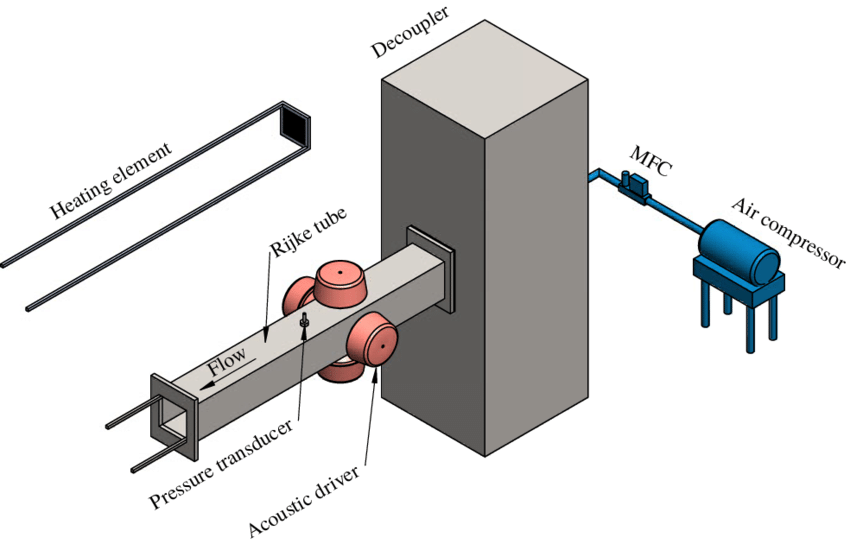
\includegraphics[width=0.5\linewidth]{setup}
    \caption{Rjike Tube Setup}
    \label{fig:setup}
\end{figure}

\section{Objective}
The model proposed to capture the dynamics exhibited by a horizontal Rijke tube is presented in the literature Balasubramanian and Sujith\cite{refpaper1} and Subramanian et al. \cite{refpaper2}. This model uses the zero Mach number approximation and is governed by the non-dimensional linearized momentum \ref{e:m} and energy \ref{e:e} equations for the acoustic field. Using the correlation provided by Heckl, it is possible to quantify how the heat transfer from the wire filament responds to changes in acoustic velocity.

We apply the RK-4 scheme after using the Galerkin technique on the ODE's we get finally for the non dimensionalised velocity and pressure to get a numerical solution to the model as explained in the following section.

\section{Methodology}

\subsection{Derivation of  Equation}
We start with the momentum and energy equation for fluids assuming that the medium is perfect and inviscid. We use $L_a$ , $L_a/c_0$, $\bar{p}$, $u_0$ and $c_0$ to non dimensionalise x, t, p',u' and $u_0$ respectively where $c_0$ is the speed of sound, $L_a$ is the duct length, $\bar{p}$ is the pressure of the undisturbed medium, and $u_0$ is the mean flow velocity. 
\begin{figure}[H]
    \centering
    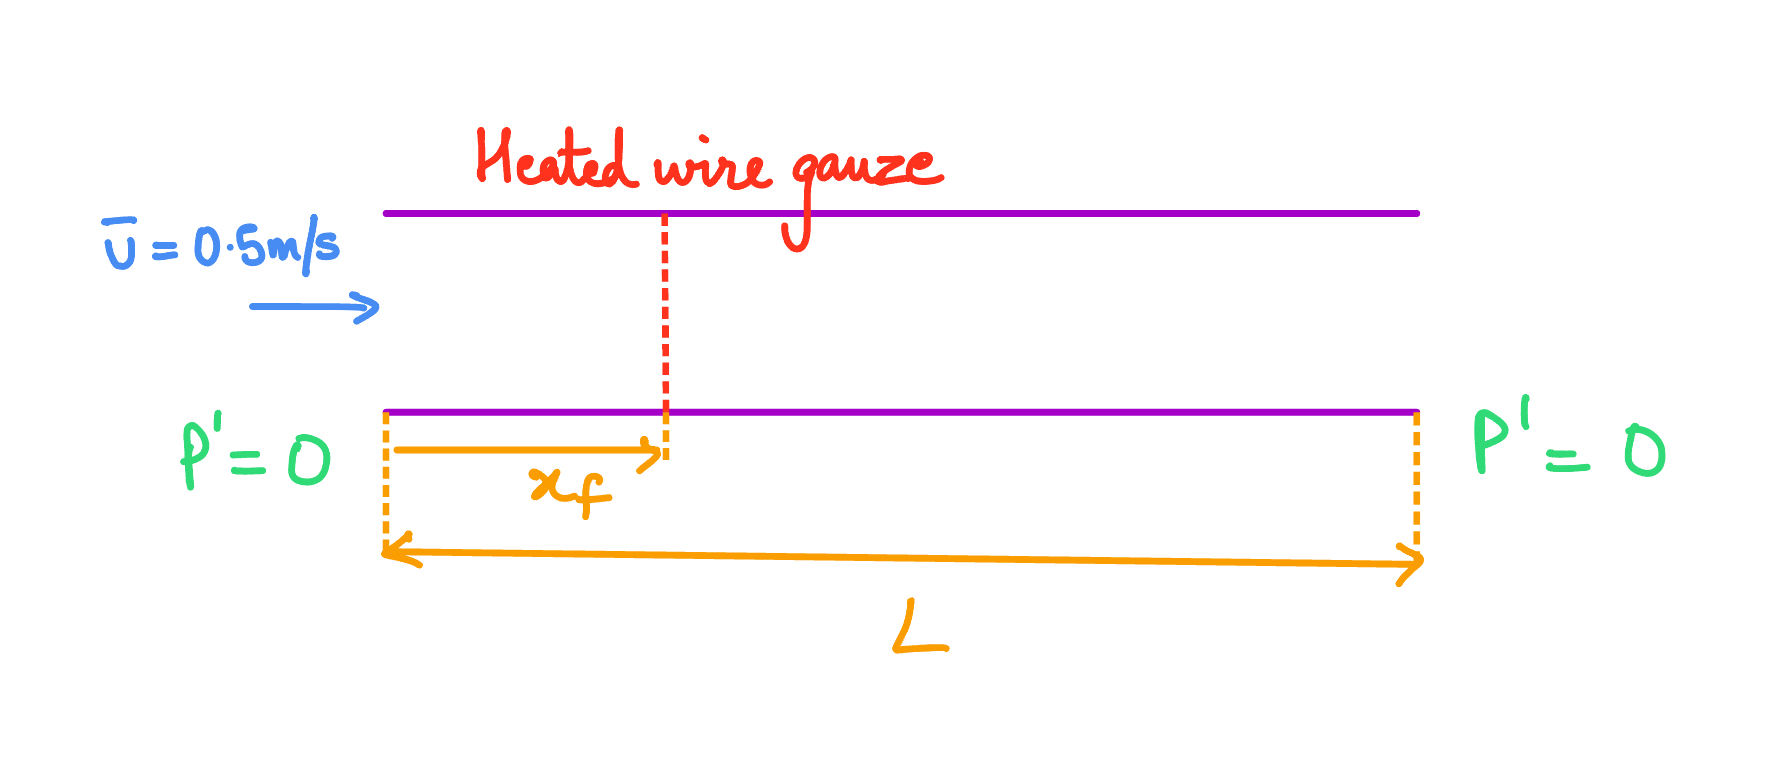
\includegraphics[width=0.4\linewidth]{schematic}
    \caption{Rjike Tube Schematic for the defined system}
    \label{fig:schematic}
\end{figure}
\noindent The linearised non-dimensional \textbf{momentum} equation in one dimension is,
\begin{equation}\label{e:m}
\gamma M \frac{\partial {u'}}{\partial {t}} + \frac{\partial {p'}}{\partial {x}} = 0
\end{equation}
and the linearised non-dimensional \textbf{energy} equation in one dimension is,
\begin{equation}\label{e:e}
\frac{\partial {p'}}{\partial {t}} + \gamma M \frac{\partial {u'}}{\partial {x}} = k \left[ \sqrt{\left| \frac{1}{3} + u'(t-\tau)\right| } - \sqrt{\frac{1}{3}} \right] \delta(x - x_f)
\end{equation}
where using a Heckl's modified form of Kings' law for heat release rate,\\
$k = \left( \gamma − 1 \right) \frac{2 L_w ( T_w − T )}{S c_0 \bar{p} \sqrt{3}} \sqrt{\pi \lambda C_v \bar{\rho} \frac{d_w}{2} u_0}$\\\\ 
$L_w$ is the equivalent length of the wire, $\lambda$ is the heat conductivity of air, $C_v$ is the specific heat of air at constant volume, $\tau$ is the time lag, $\bar{\rho}$ is the mean density of air, $d_w$ is the diameter of the wire, $T_w − T$ is the temperature difference, and S is the cross-sectional area of the duct.\\\\
The equations can be reduced to ordinary differential equations, using the Galerkin technique.
The Galerkin basis functions chosen here are the natural acoustic modes of the duct in the absence of a heater.\\
We assume the solution to p'(x,t) as,\\
\begin{center}
$p'(x,t) = \sum_{j = 1}^{N}$ $ a_j (t)$  $sin\left( j \pi x \right)  $
\end{center}
where,\\
\begin{center}
$a_j (t)$ = - $\frac{\gamma M}{j \pi} \dot{\eta_j}(t)$
\end{center}
Substituting p'(x,t) = $ \sum_{i = 1}^{N}   - \frac{\gamma M}{j \pi} \dot{\eta_j}(t) sin\left( j \pi x \right)  $ in the non dimensionalised linearised momentum equation \eqref{e:m} , we get\\
\begin{center}
$u'(x,t) = \sum_{j = 1}^{N} \eta_j (t)$ $cos\left( j \pi x \right)  $\\
\end{center}
So, from these we have $ \frac{\partial {p'(x,t)}}{\partial {t}}  =  \sum_{i = 1}^{N}   - \frac{\gamma M}{j \pi} \frac{\mathrm{d} \dot{\eta_j}(t)}{\mathrm{d} t} sin\left( j \pi x \right)  $ and $ \frac{\partial {u'(x,t)}}{\partial {x}} = \sum_{i = 1}^{N} -j \pi \eta_j (t)$ $cos\left( j \pi x \right)  $, which we substitute in the non dimensionalised linearised energy equation \eqref{e:e} , we get\\
\begin{center}
$  \sum_{j = 1}^{N}   - \frac{\gamma M}{j \pi} \frac{\mathrm{d} \dot{\eta_j}(t)}{\mathrm{d} t} sin\left( j \pi x \right)   + \gamma M  \sum_{i = 1}^{N} -j \pi \eta_j (t)$ $sin\left( j \pi x \right) =  k \left[ \sqrt{\left| \frac{1}{3} + u'(t-\tau)\right| } - \sqrt{\frac{1}{3}} \right] \delta(x - x_f) $\\
\end{center}
Multiplying both sides by $\frac{j \pi}{\gamma M}$ and shifting the summation terms to the left hand side, we get,\\
\begin{center}
$  \sum_{j = 1}^{N} \left[  \frac{\mathrm{d} \dot{\eta_j}(t)}{\mathrm{d} t}    + (-j \pi )^2  \eta_j (t) \right] sin\left( j \pi x \right) = - \frac{j \pi}{\gamma M} k \left[ \sqrt{\left| \frac{1}{3} + u'(t-\tau)\right| } - \sqrt{\frac{1}{3}} \right] \delta(x - x_f) $\\
\end{center}
$k_j$ = j $\pi$ : non-dimensionalised wave number

\subsection{Projecting along Galerkin modes (basis function)}

Multiply both sides by $sin\left( n \pi x \right)$ and integrate along the domain [0,1], to project it along nth Galerkin modes\\

$ \int_{x=0}^{x=1} \sum_{j = 1}^{N} \left[  \frac{\mathrm{d} \dot{\eta_j}(t)}{\mathrm{d} t}    + k_j^2  \eta_j (t) \right] sin\left( j \pi x \right) sin\left( n \pi x \right) \,dx   =  \int_{x=0}^{x=1} - \frac{j \pi}{\gamma M} k \left[ \sqrt{\left| \frac{1}{3} + u'(t-\tau)\right| } - \sqrt{\frac{1}{3}} \right] \delta(x - x_f) sin\left( n \pi x \right) \,dx  $\\\\
We know that,
\begin{center}
$\int_{0}^{1} sin\left( j \pi x \right) sin\left( n \pi x \right) \, dx = \frac{1}{2} \delta_{jn}$\\
$\int_{0}^{1} f(x) \delta(x - x_f) \, dx  = f(x_f)$ 
\end{center}
Thus, we get (for n=j)
\begin{center}
$   \left[  \frac{\mathrm{d} \dot{\eta_j}(t)}{\mathrm{d} t} + k_j^2  \eta_j (t) \right]  =  - \frac{j \pi}{\gamma M} k \left[ \sqrt{\left| \frac{1}{3} + u_f'(t-\tau)\right| } - \sqrt{\frac{1}{3}} \right] sin\left( j \pi x_f \right) $\\
\end{center}
\subsection{Addition of damping term}
\begin{equation}\label{e:1}
  \frac{\mathrm{d} \dot{\eta_j}(t)}{\mathrm{d} t} + 2 \zeta_j \omega_j \dot{\eta_j}  + k_j^2  \eta_j (t)  = - \frac{j \pi}{\gamma M} k \left[ \sqrt{\left| \frac{1}{3} + u_f'(t-\tau)\right| } - \sqrt{\frac{1}{3}} \right] sin\left( j \pi x_f \right) \\
\end{equation}
Frequency dependent damping : $\zeta_j = \frac{1}{2\pi} \left[ c_1 \frac{\omega_j}{\omega_1} + c_1 \sqrt{\frac{\omega_1}{\omega_j}} \right]$\\
and
\begin{equation}\label{e:2}
    \frac{\mathrm{d} \eta_j (t)}{\mathrm{d} t} = \dot{\eta_j}(t)
\end{equation}
These are the 2 final sets of equations that we obtain which we solve numerically. 

\subsection{Numerical Scheme}
For a general first order differential equation, $\frac{\mathrm{d} y(t)}{\mathrm{d} x} = f(t,y)$ , given $y(t_0) = y_0$, we wish to evolve the solution from t = $t_0$ to t = T.
The Taylor expansion of $y(t)$ around the point $t_0$ is\\\\
$y(t_0 + h) = y(t_0) + h y(t_0) + \frac{h^2}{2!} y''(t_0) \cdots$ \\\\
Neglecting the higher order terms to get Euler solution, $y(t_0 + h) = y(t_0) + h y(t_0) = y(t_0) + h f(x_0,y_0) $ \\\\
We can turn this into a basic iterative scheme as 
$y_{n+1} = y_n + h f(x_n,y_n)$ \\\\
Similarly, we simplify the equations \eqref{e:1} and \eqref{e:2} into\\
\begin{center}
$\frac{\mathrm{d} \eta_j (t)}{\mathrm{d} t} = f(t,\eta_j (t),\dot{\eta_j}(t))$\\
$\frac{\mathrm{d} \dot{\eta_j}(t)}{\mathrm{d} t} = g(t,\eta_j (t),\dot{\eta_j}(t))$
\end{center}
for j = 1,2,....n Galerkin modes.\\\\
We expand this system of equations using Taylors' expasion as shown previously. We then neglect the higher order terms according to the Runge Kutta 4th order scheme to get improved accuracy compared to Euler solution.

\subsubsection{Runge-Kutta Method}

We employ the fourth-order Runge-Kutta method using the following scheme. This numerical method is well-suited for solving ordinary differential equations (ODEs) of the form, \\$\frac{dy}{dx}$ = f(x, y),  where \( y \) is the unknown function and \( f(x, y) \) is a given function. 
\begin{center}
    $k_{1} = h f_1(t^{n}, y_{1}^n,y_{2}^n)$ \\
    $ l_1 = h f_2(t^{n}, y_{1}^n,y_{2}^n)$\\
.\\
    $k_{2} = h f_1(t^{n} + \frac{h}{2}, y_{1}^n + \frac{'k_{1}}{2}, y_{2}^n + \frac{l_{1}}{2})$\\
    $ l_2 = h f_2(t^{n} + \frac{h}{2}, y_{1}^n + \frac{k_{1}}{2}, y_{2}^n + \frac{l_{1}}{2})$ \\
.\\
    $k_{3} = h f_1(t^{n} + \frac{h}{2}, y_{1}^n + \frac{k_{2}}{2}, y_{2}^n + \frac{l_{2}}{2}) $\\
    $ l_3 =  h f_2(t^{n} + \frac{h}{2}, y^{n}_1 + \frac{k_{2}}{2}, y_{2}^n + \frac{l_{2}}{2})$ \\
.\\
    $k_{4} = h f_1(t^{n} + h, y_{1}^n + k_{3}, y_{2}^n + l_{3})$\\
    $l_4 = h f_2(t^{n} + h, y_{1}^n + k_{3}, y_{2}^n + l_{3})$ \\
\end{center}
\begin{equation}
    y^{n+1}_1 = y_{1}^n + \frac{1}{6}(k_{1} + 2k_{2} + 2k_{3} + k_{4})
\end{equation}
\begin{equation}
    y^{n+1}_2 = y_{2}^n + \frac{1}{6}(l_{1} + 2l_{2} + 2l_{3} + l_{4})
\end{equation}
where \( h \) is the step size, \( (x^{n}, y_i^{n}) \) are the current coordinates, and \( y_i^{n+1} \) are the updated coordinates.\\\\
We implement this method with boundary conditions  p'(x = 0) = 0 and p' (x = 1) = 0 to as the duct is open at both ends, as well as other initial conditions appropriately mentioned in the paper obtain the acoustic pressure \( p(x) \) throughout the duct.

\subsection{Algorithm Steps}

The steps for solving the couples ODE's with the Runge-Kutta method is:
\begin{enumerate}
    \item Initialize $\eta_j's$  and $\dot{\eta_j}'s$ as $y_1$  and $y_2$ respectively at $t = 0$.
    \item Set the fixed parameters: $x_f$, $\gamma$, M
    \item For each time step $\Delta t$, we use RK4 to get $\eta_j's$  and $\dot{\eta_j}'s$ of the next time step and use it to evaluate u'. For time $<$ $\tau$, we neglect the heat source term due to time lag and $>$ $\tau$, we include it.
    \item Store $u_{rms}$ for each K (heat source) value and/or $\tau$ (time lag) for bifurcation plots.
    \item For bifurcation plots, the initial condition for $eta_j \& \dot{eta_j}$ for next K value iteration is its the value in the last time timestep of the current time iteration.  
    \item All the data is plotted like u', $\eta_j's$, acoustic energy or bifurcation from which we take the required (the plots in the paper) plots.
\end{enumerate}

\subsection{Implementation}
The methodology was implemented in MATLAB. The code \ref{code1}\ref{code2} utilized the described algorithm to make a model to solve the system.

\section{Results}
We will now look at the results with specific system parameters and different control parameters (K) to see the variation of u' and $\eta_j$'s with time.\\
Figure. \ref{fig:4a} shows the evolution of nondimensional acoustic velocity with initial conditions of $\eta_1 (0)$ = 0.15, $x_f$ = 0:29m, K = 0.1, $\tau = 0.2s$ , $c_1$ = 0.1 and $c_2$ = 0.06 
\begin{figure}[H]
  \centering
  \begin{minipage}[b]{0.5\linewidth}
    \centering
    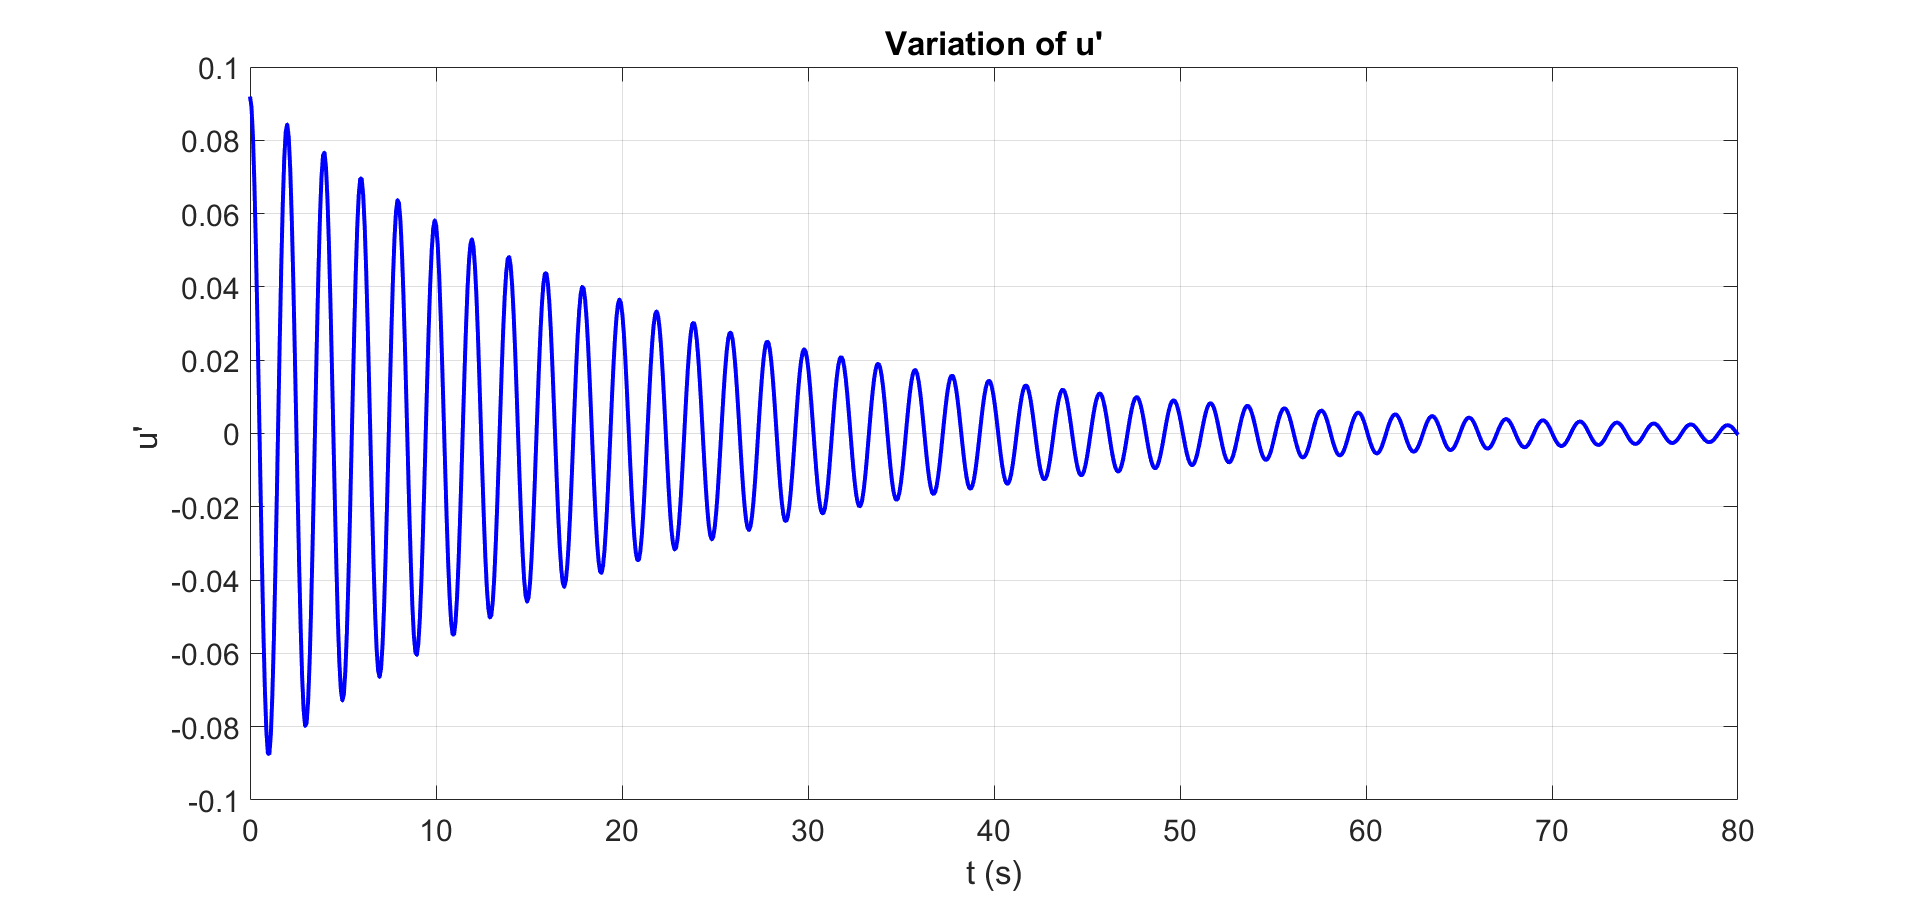
\includegraphics[width=\linewidth]{fig4a-k=0.1-tau=0.2}
   \caption{K = 0.1 ; $\tau = 0.2$; $\eta_1 (0)$ = 0.15, $\eta_{j\neq 1} (0)$ = 0 and $\dot{\eta_j} (0)$ = 0}
    \label{fig:4a}
  \end{minipage}
  \hfill
\end{figure}
It is visible that the oscillations were dampened out because the damping term predominated over the driving heat release rate. We see that the oscillations rise and saturate to high-amplitude periodic oscillations as the control parameter K is increased. Figure. \ref{fig:4b} shows the evolution of nondimensional acoustic velocity with initial conditions of $\eta_1 (0)$ = 0.15, $x_f$ = 0:29m, K = 0.1, $\tau = 0.5s$ , $c_1$ = 0.1 and $c_2$ = 0.06 
\begin{figure}[H]
  \centering
  \begin{minipage}[b]{0.495\linewidth}
    \centering
    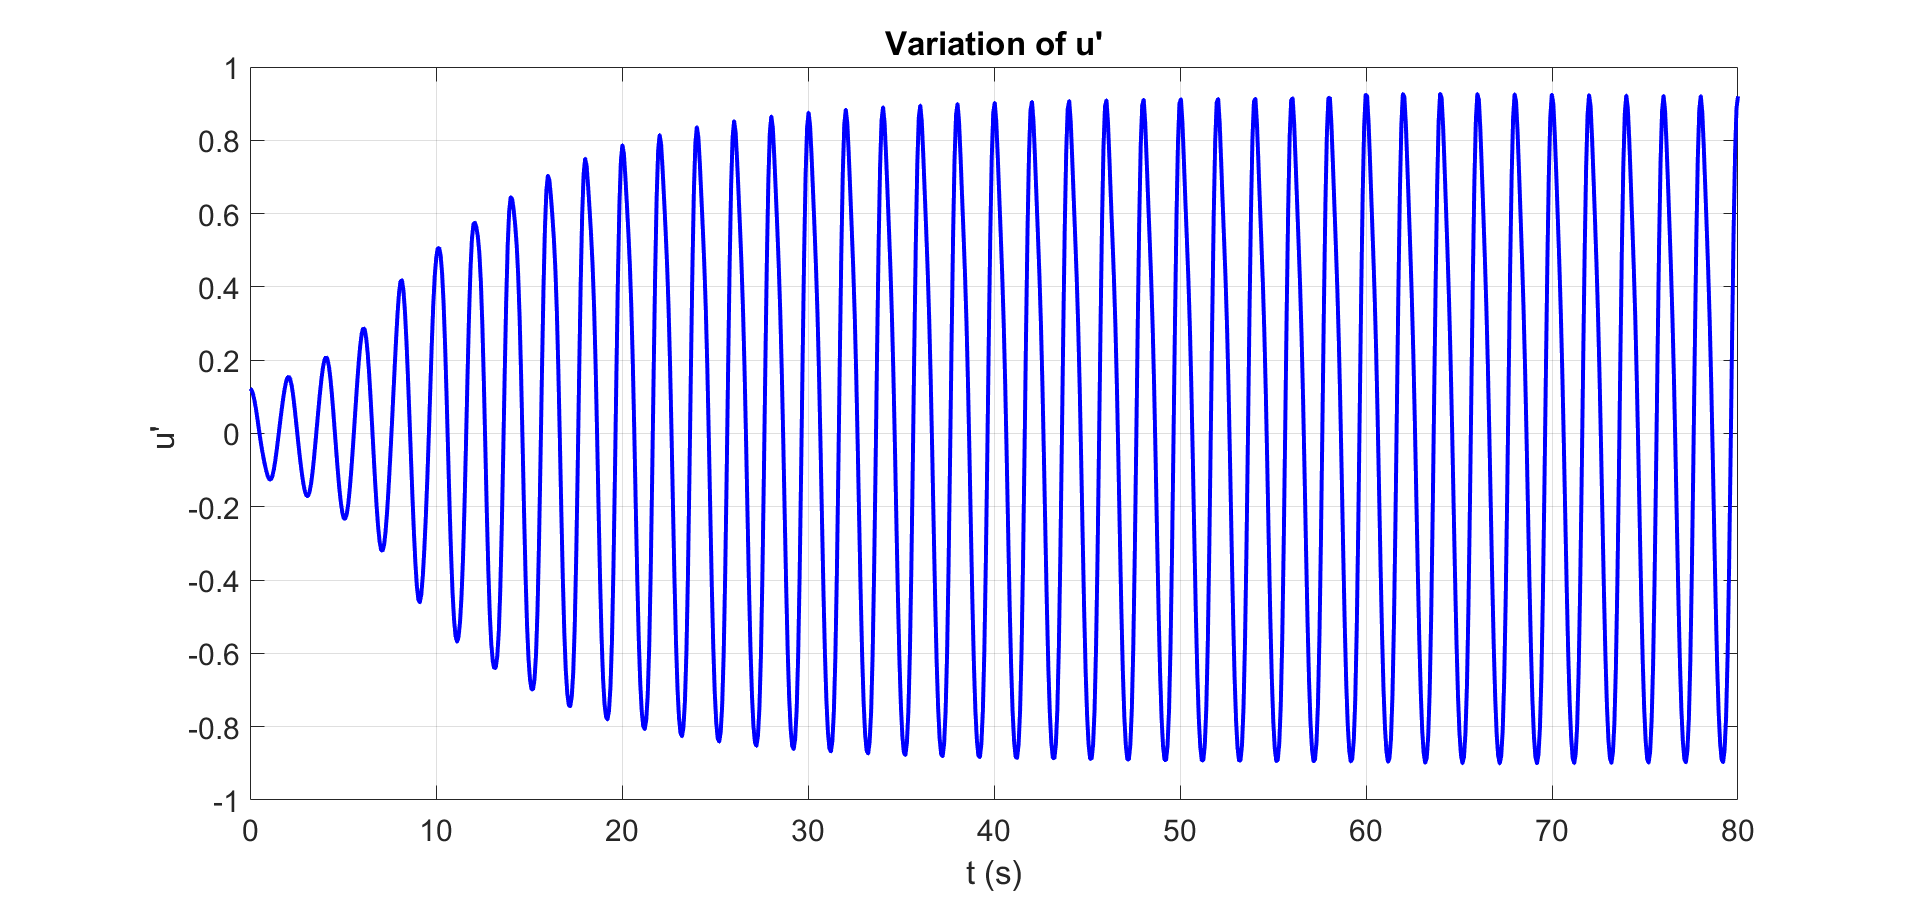
\includegraphics[width=\linewidth]{fig4b-k=0.6-tau=0.5}
   \caption{Velocity Fluctuations}
    \label{fig:4b}
  \end{minipage}
  \hfill
  \begin{minipage}[b]{0.495\linewidth}
    \centering
    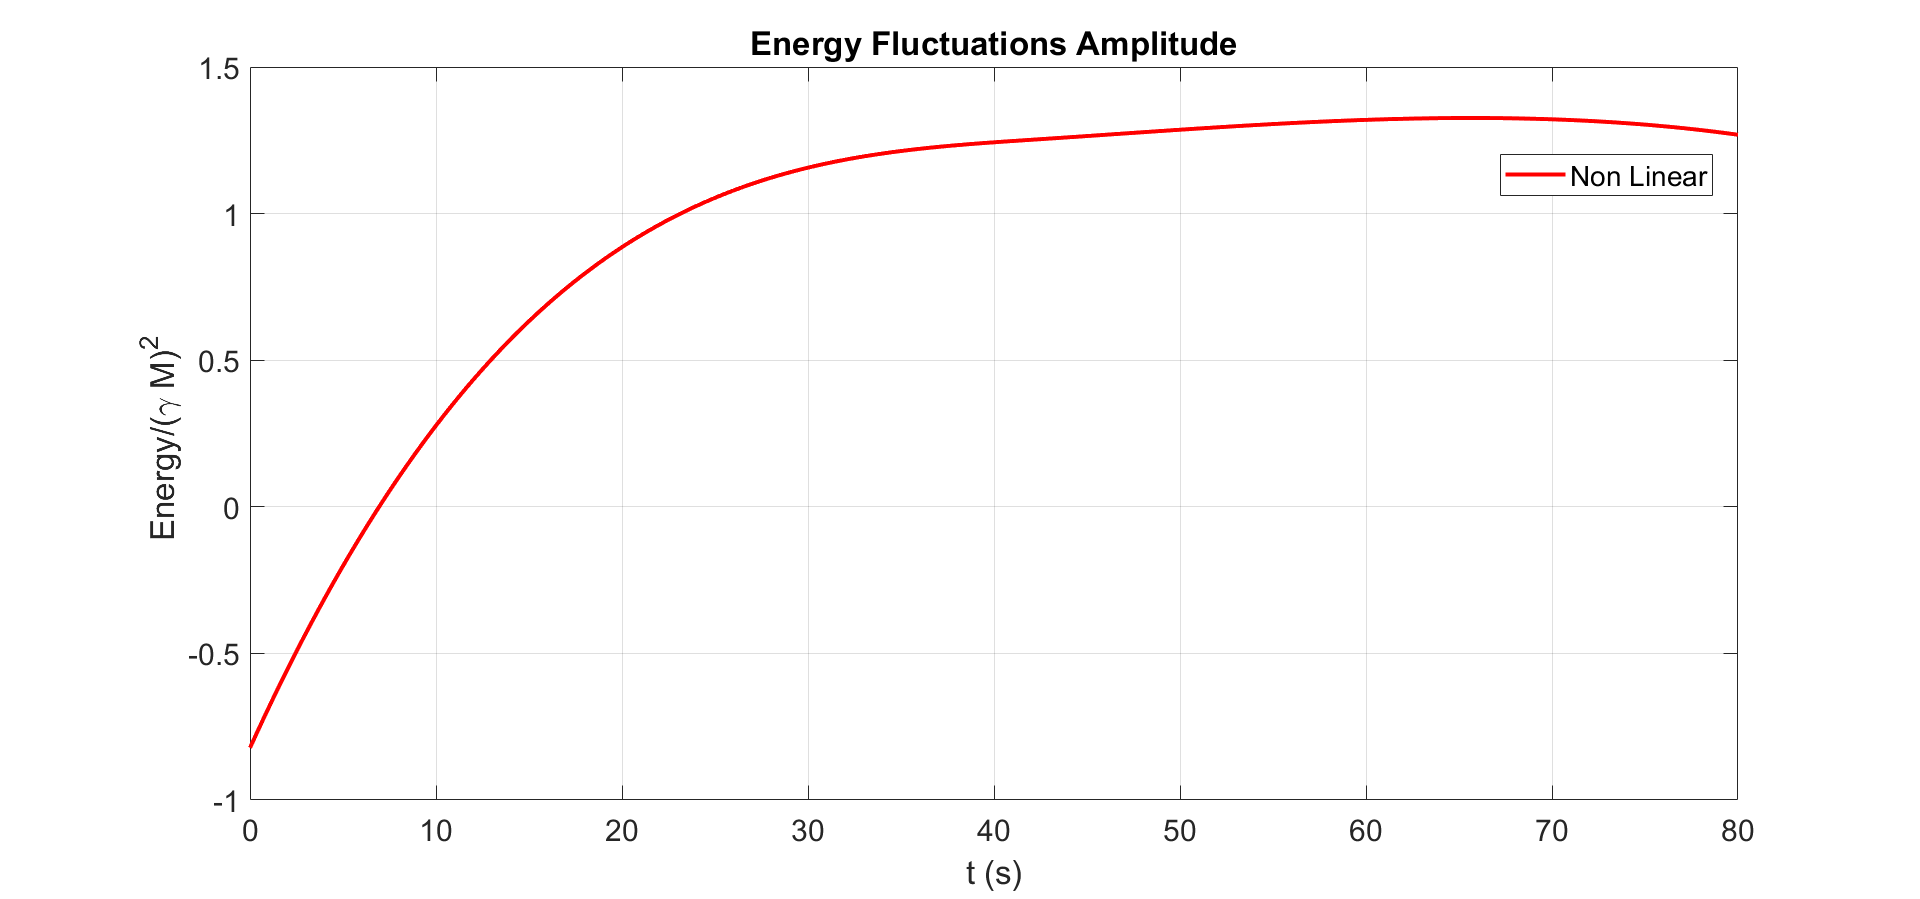
\includegraphics[width=\linewidth]{fig4d-k=0.6-tau=0.5}
    \caption{Energy}
    \label{fig:4d}
  \end{minipage}
\caption*{K = 0.6 ; $\tau = 0.5$; $\eta_1$ = 0.2, $\eta_{j\neq 1}$ = 0 and $\dot{\eta_j}$ = 0}
\end{figure}
Here, the driving term of the heat release is dominant and increase the amplitude of the oscillations. The growth of the system is further inhibited with the non-linearities in the system.\\
The non-dimensional acoustic energy is defined as:
\begin{equation}
	E = \frac{1}{(\gamma M)^2} \left( \frac{1}{2} p'^2 + \frac{1}{2} (\gamma M u')^2 \right)
\end{equation}
As the oscillations also grow in the second case, we would expect the energy also to grow,
which is clearly seen in the numerical result (Fig. \ref{fig:4d}).\\
We look at the variation of $u'$, $\eta_1 (t)$, $\eta_2 (t)$  and $\eta_3 (t)$ for different K and $\tau$ value for a different initial condition as mentioned with the figures (Fig.\ref{fig:fig5} and Fig.\ref{fig:fig6})
\begin{figure}[H]
    \centering
    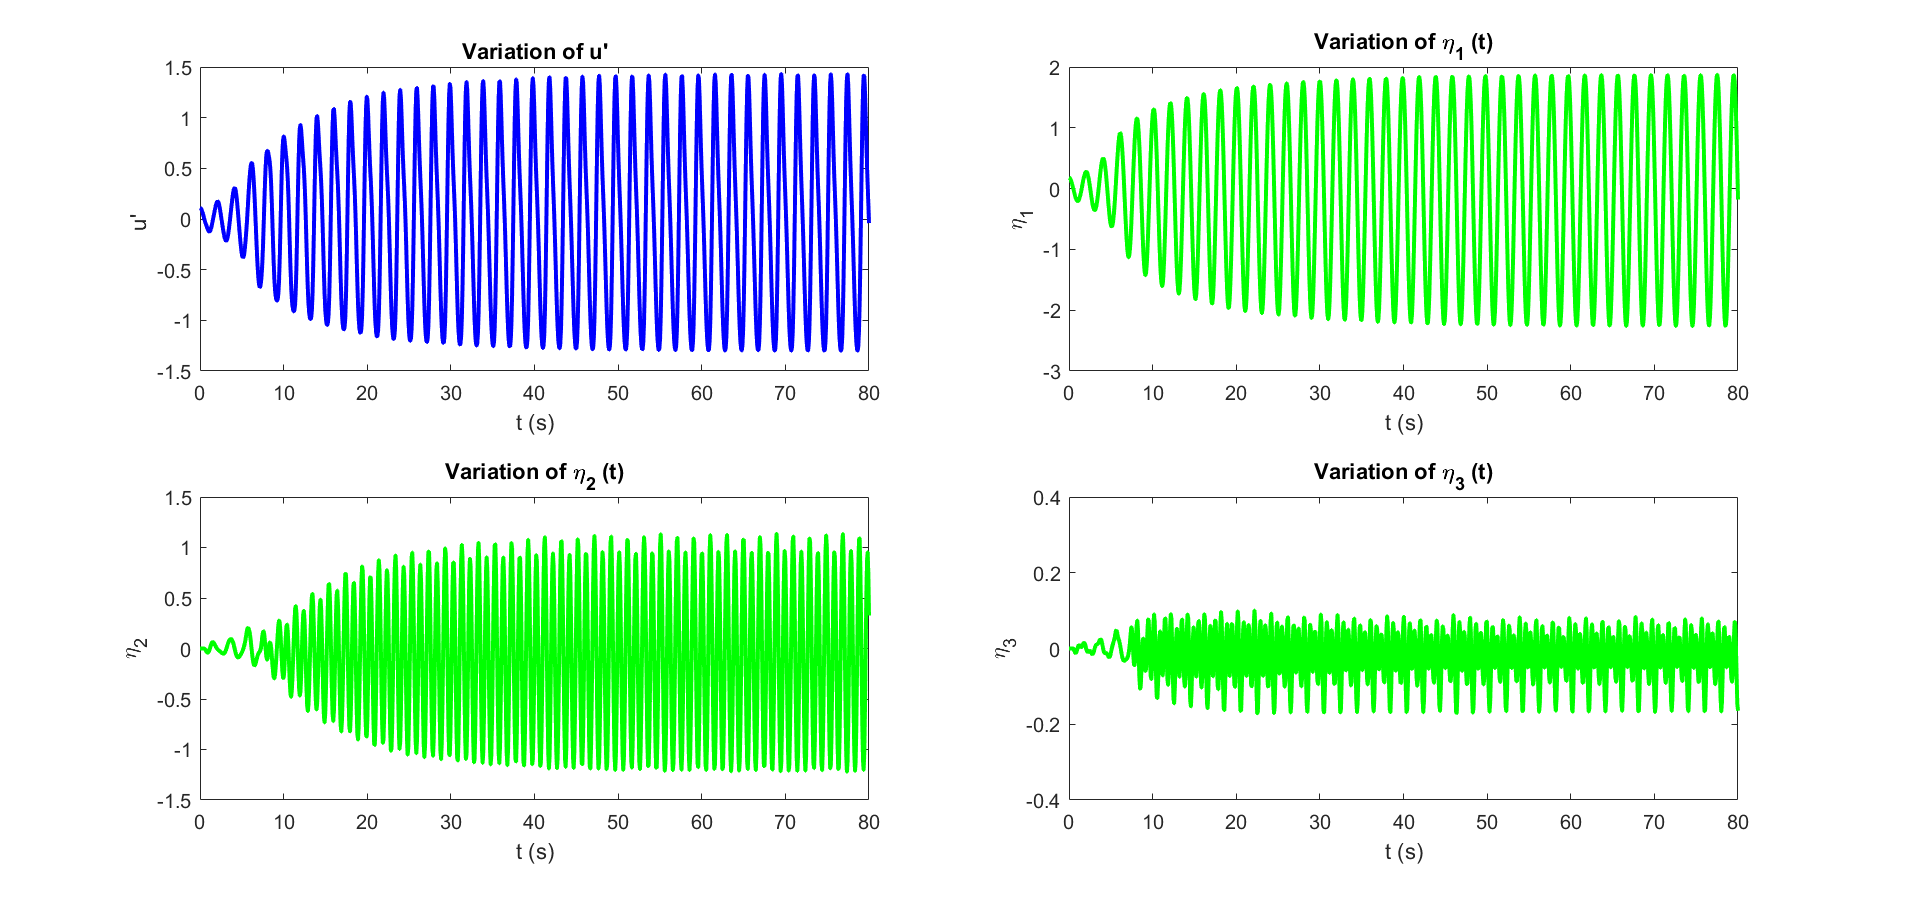
\includegraphics[width=\linewidth]{fig5-k=1-tau=0.5}
    \caption{K = 1 ; $\tau = 0.5$; $\eta_1$ = 0.18, $\eta_{j\neq 1}$ 0 and $\dot{\eta_j}$ = 0}'
    \label{fig:fig5}
\end{figure}
We see that the amplitude of u' and its 3 Galerkin modes grows in Fig.\ref{fig:fig5}  and decays in Fig.\ref{fig:fig6}. 
\begin{figure}[H]
    \centering
    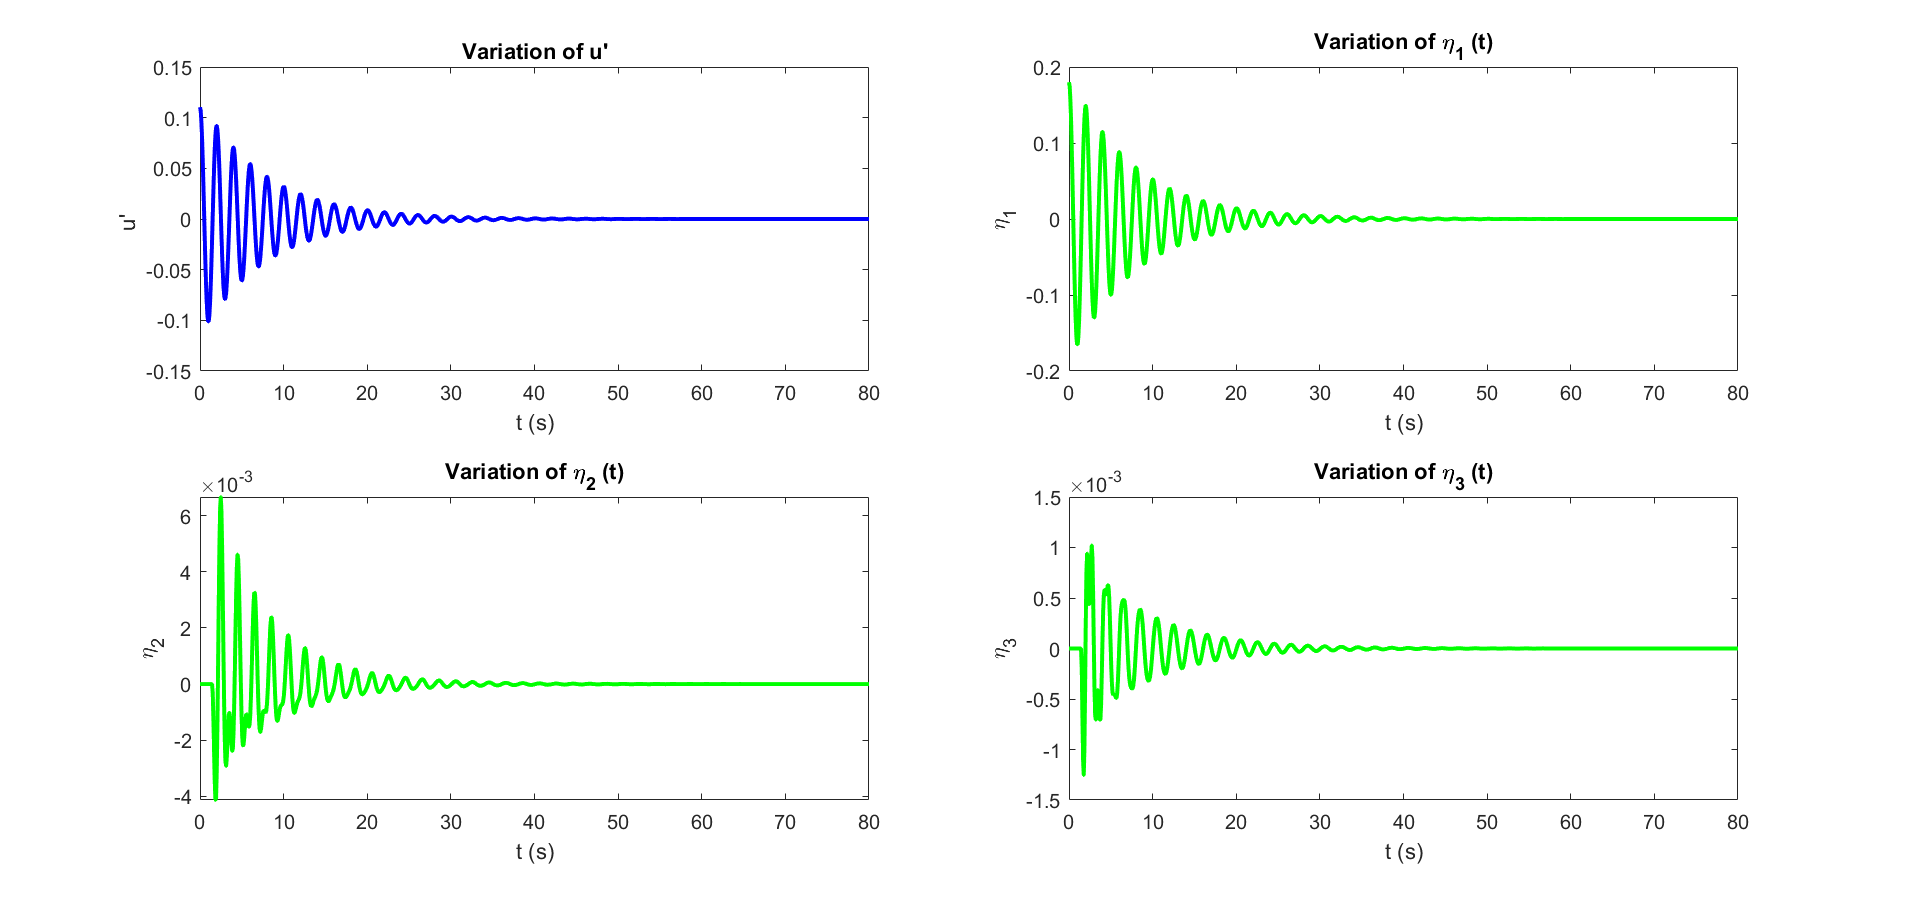
\includegraphics[width=\linewidth]{fig6}
     \caption{K = 0.3 ; $\tau = 0.45\pi$; $\eta_1 (0)$ = 0.18, $\eta_{j\neq 1} (0)$ = 0 and $\dot{\eta_j} (0)$ = 0}
    \label{fig:fig6}
\end{figure}
Now, we vary the control parameter to capture the change in the dynamics of this nonlinear system. The control parameter K is varied from 0.2 to 1.4 keeping $\tau$ = 0.2, $c_1$ = 0.01 and $c_2$ = 0.06 constant. We can see the evolution of $|u'|$, the non-dimensional acoustic velocity with changing K for a single Galerkin mode in Fig. \ref{fig:bifur}.\\
Below approximately K $<$ 0.8, we see the system to dampen out. When the oscillations increased in amplitude above this control value, they reached a state of thermoacoustic instability. Since periodic dynamics abruptly emerge from an initial state at this point, it is also known as the \textbf{Hopf point} and the dynamics is said to undergo subcritical Hopf bifurcation. $|U_1|$ exhibits hysteresis at the point of instability (red data points in Fig. \ref{fig:bifur}) when the control parameter is reversed from K = 1.4.
\begin{figure}[H]
  \centering
    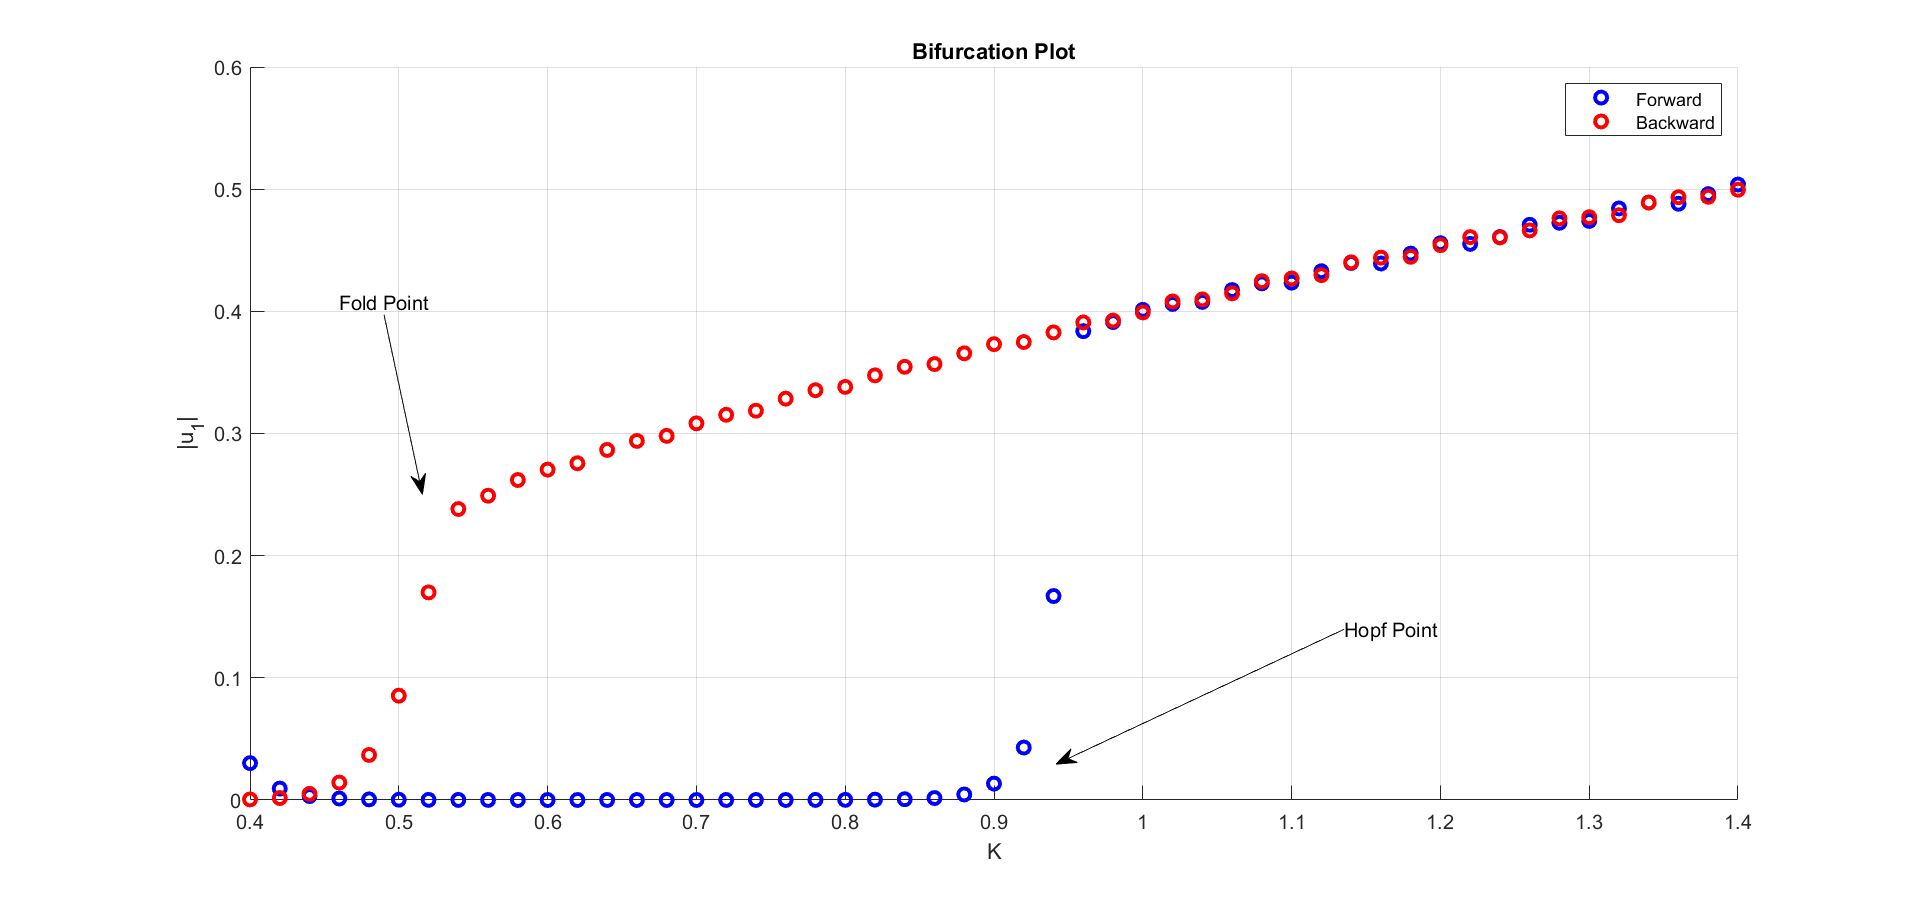
\includegraphics[width=0.9\linewidth]{bifur}
   \caption{Bifurcation plot for variation of non-dimensional heater power K}
    \label{fig:bifur}
\end{figure}
\noindent Lastly, we also plot the bifurcation diagram to observe the system behaviour for different time lag for a single Galerkin mode. The 3D plot of bifurcation plot of non-dimensional heater power K for varying values of time lag $\tau$ with the other parameters of the system $c_1$ = 0.01, $c_2$ = 0.06 and $x_f$ = 0.29m is shown in Fig. \ref{fig:3dbifur}.
\begin{figure}[H]
  \centering
    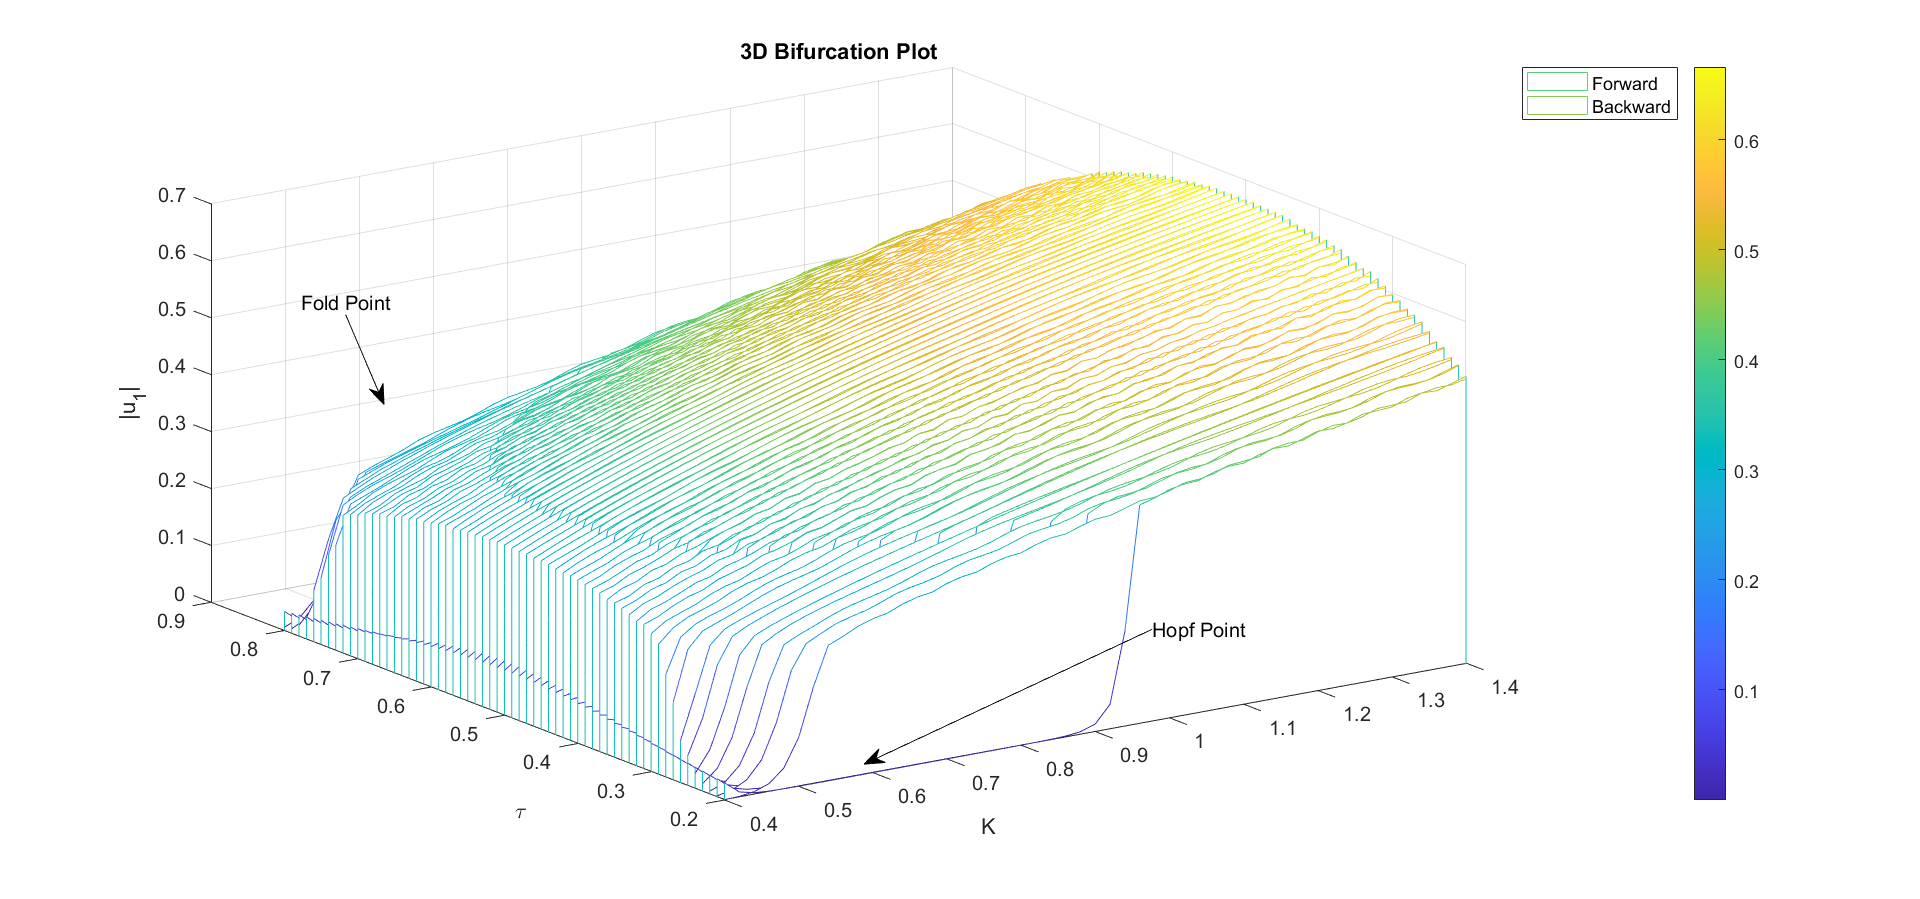
\includegraphics[width=1\linewidth]{bifur_3d}
   \caption{3D Bifurcation Plot for variation of K and $\tau$}
    \label{fig:3dbifur}
\end{figure}

\section{Summary}
A model for a horizontal Rijke tube's dynamic behaviour has been examined using the numerical continuation approach. It is seen that the model selected to mimic the Rijke tube's activity depicts the results for subcritical Hopf bifurcations. In conclusion, in order to identify stability limits, produce bifurcation maps, and evaluate possible dynamical behaviour, the numerical continuation approach can be applied to a full analysis of reduced order models of physical systems with explicit time delays.

\section{References}
\begin{thebibliography}{99}

\bibitem{refpaper1}
Non-normality and nonlinearity in combustion–acoustic interaction in diffusion flames\\ \url{https://www.cambridge.org/core/services/aop-cambridge-core/content/view/F6874EEEE2B1EDD0ACA05320FD6C3701/S0022112007008737a.pdf/nonnormality_and_nonlinearity_in_combustionacoustic_interaction_in_diffusion_flames.pdf}
\bibitem{refpaper2}
Bifurcation analysis of thermoacoustic
instability in a horizontal Rijke tube\\ \url{https://www.researchgate.net/publication/265794610_Bifurcation_Analysis_of_Thermoacoustic_Instability_in_a_Horizontal_Rijke_Tube}

\end{thebibliography}

\newpage
\section{Appendix}

\subsection{u' and it's $\eta_j$ $\&$ $\dot{\eta_j}$ Code}\label{code1}
\begin{lstlisting}
N =1000; %number of timesteps
%T = 40; %total time of experiment %fig4a,4b,4c
T = 80; %total time of experiment %fig5a,5b,5c,5d fig6a,6b,6c,6d
dt = (T/N);

%define system parameters
g = 1.4;
c0 = 399.6; %speed of sound
u0 = 0.5; %mean velocity of air
M = u0/c0;

K = 0.1 %fig4a
%K = 0.6 %fig4b,4d
%K = 1 %fig5a,5b,5c,5d
%K = 0.1 %fig6a,6b,6c,6d

xf = 0.29 %fig4a,4b,4d %fig5a,5b,5c,5d fig6a,6b,6c,6d

tau = 0.2 %fig4a
%tau = 0.5 %fig4b,4d
%tau = 0.5 %fig5a,5b,5c,5d 
%tau = 0.45*pi % fig6a,6b,6c,6d

% Set initial values
u = zeros(1, N);
p = zeros(1, N);

J = 3 %number of Galerkin modes

% Preallocate arrays
y1 = zeros(J, N);
y2 = zeros(J, N);
% Set initial values
y1(:,1) = 0;
y1(1,1) = 0.15 %fig4a
%y1(1,1) = 0.2; %fig4b,4d
%y1(1,1) = 0.18; %fig5a,5b,5c,5d fig6a,6b,6c,6d
y2(:,1) = 0;
u(1) = y1(1,1)*cos(pi*xf);
p(1) = 0;        

n1 = round(tau/dt);
% Fourth-order Runge-Kutta method
% for t < tau
for n = 1:n1   
    for j=1:J    
        [k1, l1] = equations1(y1(j,n), y2(j,n),j);
        [k2, l2] = equations1(y1(j,n) + 0.5*dt*k1, y2(j,n) + 0.5*dt*l1,j);
        [k3, l3] = equations1(y1(j,n) + 0.5*dt*k2, y2(j,n) + 0.5*dt*l2,j);
        [k4, l4] = equations1(y1(j,n) + dt*k3, y2(j,n) + dt*l3,j);
    
        y1(j,n+1) = y1(j,n) + (dt/6) * (k1 + 2*k2 + 2*k3 + k4);
        y2(j,n+1) = y2(j,n) + (dt/6) * (l1 + 2*l2 + 2*l3 + l4);
    
        u(n+1) = u(n+1) + y1(j,n+1)*cos(j*pi*xf);
        p(n+1) = p(n+1) + y2(j,n+1)*((-g*M)/(j*pi))*sin(j*pi*xf);
    end
end
% for t > tau
for n = n1+1:N-1
    for j=1:J
        [k1, l1] = equations2(y1(j,n), y2(j,n),j,K,u(n-n1),xf);
        [k2, l2] = equations2(y1(j,n) + 0.5*dt*k1, y2(j,n) + 0.5*dt*l1,j,K,u(n-n1),xf);
        [k3, l3] = equations2(y1(j,n) + 0.5*dt*k2, y2(j,n) + 0.5*dt*l2,j,K,u(n-n1),xf);
        [k4, l4] = equations2(y1(j,n) + dt*k3, y2(j,n) + dt*l3,j,K,u(n-n1),xf);
    
        y1(j,n+1) = y1(j,n) + (dt/6) * (k1 + 2*k2 + 2*k3 + k4);
        y2(j,n+1) = y2(j,n) + (dt/6) * (l1 + 2*l2 + 2*l3 + l4);
    
        u(n+1) = u(n+1) + y1(j,n+1)*cos(j*pi*xf);
        p(n+1) = p(n+1) + y2(j,n+1)*((-g*M)/(j*pi))*sin(j*pi*xf);
    end
end       


figure(1);
plot(linspace(0,T,N), u, 'b','linewidth',2);
title('Variation of u''');
xlabel('t (s)');
ylabel('u'' ');
fontsize(gcf,scale=1.5)
grid on;

e=((0.5*(p.^2)+0.5*(g*M*u).^2)/((g*M)^2));
ee = envelope(e,200,"peak");
figure(5);
plot(linspace(0,T,N), ee, 'r','linewidth',2);
title('Energy Fluctuations Amplitude');
xlabel('t (s)');
ylabel('Energy/(\gamma M)^2 ');
legend('Non Linear')
fontsize(gcf,scale=1.5)
grid on;

figure(2);
plot(linspace(0,T,N), y1(1,:), 'm','linewidth',2);
xlabel('t (s)');
ylabel('\eta_1');
title('Variation of \eta_1 (t)');
fontsize(gcf,scale=1.5)
grid on;

figure(3);
plot(linspace(0,T,N), y1(2,:), 'm','linewidth',2);
xlabel('t (s)');
ylabel('Variation of \eta_2');
title('\eta_2 (t)');
fontsize(gcf,scale=1.5)
grid on;

figure(4);
plot(linspace(0,T,N), y1(3,:), 'm','linewidth',2);
xlabel('t (s)');
ylabel('\eta_3');
title('Variation of  \eta_3 (t)');
fontsize(gcf,scale=1.5)
grid on;

%combined plot
figure(6)
tiledlayout(2,2)
nexttile
plot(linspace(0,T,N), u, 'b','linewidth',2);
title('Variation of u''');
xlabel('t (s)');
ylabel('u'' ');
nexttile
plot(linspace(0,T,N), y1(1,:), 'g','linewidth',2);
xlabel('t (s)');
ylabel('\eta_1');
title('Variation of \eta_1 (t)');
nexttile
plot(linspace(0,T,N), y1(2,:), 'g','linewidth',2);
xlabel('t (s)');
ylabel('\eta_2');
title('Variation of \eta_2 (t)');
nexttile
plot(linspace(0,T,N), y1(3,:), 'g','linewidth',2);
xlabel('t (s)');
ylabel('\eta_3');
ylim([-0.4 0.4])
title('Variation of \eta_3 (t)');


% Define the functions f1(x, y1, y2) and f2(x, y1, y2) 
% where y1 is eta and y2 is eta dot

% for t < tau
function [f1,f2] = equations1(y1, y2, j)
    kj = j*pi;
    wj = kj;
    w1 = pi;
    c1 = 0.1; c2 = 0.06;
    zetaj = (1/(2*pi))*(c1*(wj/w1) + c2*sqrt(w1/wj));
    
    f1 =  y2;
    f2 =  - (kj^2) * y1 - 2*zetaj*wj*y2;
end

% for t > tau
function [f1,f2] = equations2(y1, y2, j, K, u,xf)
    kj = j*pi;
    wj = kj;
    w1 = pi;
    c1 = 0.1; c2 = 0.06;
    zetaj = (1/(2*pi))*(c1*(wj/w1) + c2*sqrt(w1/wj));

    f1 =  y2;
    f2 = - (kj^2) * y1 - 2*zetaj*wj*y2 - ((2*j*pi*K))*(sqrt(abs((1/3) + u)) - sqrt(1/3))*sin(j*pi*xf) ;
end


\end{lstlisting}

\subsection{Bifurcation Code}\label{code2}
\begin{lstlisting}
N = 1000; %number of timesteps
T = 40; %total time of experiment
dt = (T/N);
xf = 0.3; %m

%define system parameters
g = 1.4;
c0 = 399.6; %speed of sound
u0 = 0.5; %mean velocity of air
M = u0/c0;

J = 3; %number of Galerkin modes

% Set initial values
ks=0.2:0.01:1.4;%non-dimensional heater power
n1=length(ks)

tau=0.2:0.01:0.8;%time-lag
n3=length(tau)

% Preallocate arrays
u_rms1 = zeros(n3,n1);

y1 = zeros(n3,J, N);
y2 = zeros(n3,J, N);

%forward
for i=1:n3
    y1(i,1,1)=0.18;
    u1 = zeros(n1, N);
    for k=1:n1
        % Set initial values
        for j = 1:J
            u1(k,1) = u1(k,1) + y1(i,j,1)*cos(j*pi*xf);
        end
            
        n2 = round(tau(i)/dt);
        % Fourth-order Runge-Kutta method
        for n = 1:n2   
          for j=1:J
            [k1, l1] = equations1(y1(i,j,n), y2(i,j,n),j);
            [k2, l2] = equations1(y1(i,j,n) + 0.5*dt*k1, y2(i,j,n) + 0.5*dt*l1,j);
            [k3, l3] = equations1(y1(i,j,n) + 0.5*dt*k2, y2(i,j,n) + 0.5*dt*l2,j);
            [k4, l4] = equations1(y1(i,j,n) + dt*k3, y2(i,j,n) + dt*l3,j);
        
            y1(i,j,n+1) = y1(i,j,n) + (dt/6) * (k1 + 2*k2 + 2*k3 + k4);
            y2(i,j,n+1) = y2(i,j,n) + (dt/6) * (l1 + 2*l2 + 2*l3 + l4);
    
            u1(k,n+1) = u1(k,n+1) + y1(i,j,n+1)*cos(j*pi*xf);
          end
        end
    
        for n = n2+1:N-1
          for j=1:J
            [k1, l1] = equations2(y1(i,j,n), y2(i,j,n),j,ks(k),u1(k,n-n2),xf);
            [k2, l2] = equations2(y1(i,j,n) + 0.5*dt*k1, y2(i,j,n) + 0.5*dt*l1,j,ks(k),u1(k,n-n2),xf);
            [k3, l3] = equations2(y1(i,j,n) + 0.5*dt*k2, y2(i,j,n) + 0.5*dt*l2,j,ks(k),u1(k,n-n2),xf);
            [k4, l4] = equations2(y1(i,j,n) + dt*k3, y2(i,j,n) + dt*l3,j,ks(k),u1(k,n-n2),xf);
        
            y1(i,j,n+1) = y1(i,j,n) + (dt/6) * (k1 + 2*k2 + 2*k3 + k4);
            y2(i,j,n+1) = y2(i,j,n) + (dt/6) * (l1 + 2*l2 + 2*l3 + l4);
    
            u1(k,n+1) = u1(k,n+1) + y1(i,j,n+1)*cos(j*pi*xf);
          end
        end

        %figure(k);
        %plot(0:N-1, u1(k,:), 'k','linewidth',2);
        %xlabel('t');
        %ylabel('|u''|');
        %grid on;

        %getting initial values for next
        y1(i,:,1) = y1(i,:,N);
        y2(i,:,1) = y2(i,:,N);     
    
        u_rms1(i,k) = rms(u1(k,:));
    end
end

% Preallocate arrays
u_rms2 = zeros(n3,n1);

%backward 
for i=1:n3
    u2 = zeros(n1, N);
    for k=1:n1
        % Set initial values
        for j=1:j
            u2(n1-k+1,1) = u2(n1-k+1,1) + y1(i,j,1)*cos(j*pi*xf);
        end

        n2 = round(tau(i)/dt);
        % Fourth-order Runge-Kutta method
        for n = 1:n2    
          for j=1:J
            [k1, l1] = equations1(y1(i,j,n), y2(i,j,n),j);
            [k2, l2] = equations1(y1(i,j,n) + 0.5*dt*k1, y2(i,j,n) + 0.5*dt*l1,j);
            [k3, l3] = equations1(y1(i,j,n) + 0.5*dt*k2, y2(i,j,n) + 0.5*dt*l2,j);
            [k4, l4] = equations1(y1(i,j,n) + dt*k3, y2(i,j,n) + dt*l3,j);
        
            y1(i,j,n+1) = y1(i,j,n) + (dt/6) * (k1 + 2*k2 + 2*k3 + k4);
            y2(i,j,n+1) = y2(i,j,n) + (dt/6) * (l1 + 2*l2 + 2*l3 + l4);
    
            u2(n1-k+1,n+1) = u2(n1-k+1,n+1) + y1(i,j,n+1)*cos(j*pi*xf);
          end
        end
    
        for n = n2+1:N-1
          for j=1:J
            [k1, l1] = equations2(y1(i,j,n), y2(i,j,n),j,ks(n1-k+1),u2(n1-k+1,n-n2),xf);
            [k2, l2] = equations2(y1(i,j,n) + 0.5*dt*k1, y2(i,j,n) + 0.5*dt*l1,j,ks(n1-k+1),u2(n1-k+1,n-n2),xf);
            [k3, l3] = equations2(y1(i,j,n) + 0.5*dt*k2, y2(i,j,n) + 0.5*dt*l2,j,ks(n1-k+1),u2(n1-k+1,n-n2),xf);
            [k4, l4] = equations2(y1(i,j,n) + dt*k3, y2(i,j,n) + dt*l3,j,ks(n1-k+1),u2(n1-k+1,n-n2),xf);
        
            y1(i,j,n+1) = y1(i,j,n) + (dt/6) * (k1 + 2*k2 + 2*k3 + k4);
            y2(i,j,n+1) = y2(i,j,n) + (dt/6) * (l1 + 2*l2 + 2*l3 + l4);
    
            u2(n1-k+1,n+1) = u2(n1-k+1,n+1) + y1(i,j,n+1)*cos(j*pi*xf);
          end
        end

        %figure(k);
        %plot(0:N-1, u2(k,:), 'k','linewidth',2);
        %xlabel('t');
        %ylabel('|u''|');
        %grid on;

        %getting initial values
        y1(i,:,1) = y1(i,:,N);
        y2(i,:,1) = y2(i,:,N);
 
        u_rms2(i,n1-k+1) = rms(u2(n1-k+1,:));
    end
end

for i=1:n3
    if tau(i)==0.2
        figure(1);
        scatter(ks,u_rms1(i,:),'b','linewidth',2);
        hold on;
        scatter(ks,u_rms2(i,:),'r','linewidth',2);
        xlabel('K');
        ylabel('|u_1|');
        legend('Forward','Backward')
        title('Bifurcation Plot')
        annotation('textarrow',[0.7 0.6],[0.3 0.15],'String','Hopf Bifurcation')
        annotation('textarrow',[0.25 0.3],[0.65 0.55],'String','Fold Bifurcation')
        grid on;
    end
end


figure(2);
mesh(u_rms1);
mesh(u_rms2);
C = gradient(u_rms1);
waterfall(ks,tau,u_rms1);
hold on;
waterfall(ks,tau,u_rms2);
xlabel('K')
ylabel('tau');
zlabel('|u_1|')
legend('Forward','Backward')
title('3D Bifurcation Plot')
annotation('textarrow',[0.6 0.45],[0.3 0.15],'String','Hopf Bifurcation')
annotation('textarrow',[0.2 0.25],[0.6 0.5],'String','Fold Bifurcation')
colorbar

% Define the functions f1(x, y1, y2) and f2(x, y1, y2) 
% where y1 is eta and y2 is eta dot

% for t < tau
function [f1,f2] = equations1(y1, y2, j)
    kj = j*pi;
    wj = kj;
    w1 = pi;
    c1 = 0.1; c2 = 0.06;
    zetaj = (1/(2*pi))*(c1*(wj/w1) + c2*sqrt(w1/wj));
    
    f1 =  y2;
    f2 = -2*zetaj*wj*y2 - (kj^2) * y1;
end

% for t > tau
function [f1,f2] = equations2(y1, y2, j, K, u,xf)
    kj = j*pi;
    wj = kj;
    w1 = pi;
    c1 = 0.1; c2 = 0.06;
    zetaj = (1/(2*pi))*(c1*(wj/w1) + c2*sqrt(w1/wj));

    f1 =  y2;
    f2 = -2*zetaj*wj*y2 - (kj^2) * y1 - j*pi*K*(abs(sqrt((1/3) + u)) - sqrt(1/3))*sin(j*pi*xf) ;
end
\end{lstlisting}



\end{document}